\documentclass[./\jobname.tex]{subfiles}
\begin{document}
\chapter {Experiment 2: Adaptive Number of Kernels}
\label{chap:experimet_2}

Although, the parallel algorithm is effectively faster, the quality of the achieved solution is still not good enough. A common inaccuracy, especially with the testbed \gls{pde} 0A is, that the not all Gauss ``bumps'' are represented in the approximation, as described in chapter \ref{chap: experiment_0_pde_0A}. A possible method to compensate that could be to adapte the number of kernels along the solving process, instead of arbitrarily using 5 kernels. 

\section{Hypotheses}

The idea that this chapter tests is an adaptive scheme for the number of kernels used, which is directly linked to the search dimensionality of the optimisation problem. 

This new concept requires a convergence based halting criterion in the JADE algorithm, which is not included in the original algorithm. The pseudocode \ref{algo: pajade} in the appendix \ref{chap:pseudocode_pajade} is extended by a so called state detector. Ideally, the lines 37 to 40 should stop the overall optimisation loop as soon as the algorithm has converged and before the function evaluation budget is exceeded. Generally, this is done by checking if the function value has not changed for a certain amount of generations. The state detector introduces a new parameters: the \gls{dt}, which represents the number of generations that the best function value must stay the same. It can also be thought of a buffer-time that allows the \gls{de} parameters F and CR to self-adapt. Further, the minError parameter has a new purpose: this is the minimal difference that the value is allowed to change over \gls{dt} generations. 

The new paJADE is wrapped into the memetic framework, already used in the chapters before. The new algorithm \ref{algo: memeticpJADEadaptive} is shown below, which also describes the kernel number adaption. Whenever a JADE/\gls{ds} cycle is concluded, it is checked if the resulting function value is better than the previous best function value. If the new result is better (line 17), the problem dimensionality is increased by one kernel (line 19). Since the dimension is greater, the population size must be adapted by the same factor (line 20). If the function value could not be surpassed, a restart around the previous best value solution is performed (line 27). Thus, the dimension can increase one kernel at a time, but it can only fall back one kernel. 


\begin{algorithm}[H]
	\SetAlgoNoLine
	\DontPrintSemicolon
	\SetKwFunction{FmpJADE}{memeticpJADE}
	\SetKwProg{Fn}{Function}{:}{}
	\Fn{\FmJADE{$\mathbf{X}$, $funct$, $minErr$, $maxFE$}}{
		$dim$, $popsize$, $kernelsize$ $\gets size(\mathbf{X})$\;
		$p \gets 0.3$\;
		$c \gets 0.5$\;
		$delayTime$ $\gets 100$\;
		$fecounter \gets 0$\;
		$bestFE \gets \inf$\;
		$bestPop \gets \emptyset$\;
		$popFactor$ $\gets$ $psize/dim$\;
		\While{$fecounter < maxFE$}{
			$pop$, $FE$, $F$, $CR$ $\gets paJADE($$\mathbf{X}$, $p$, $c$, $dT$, $funct$, $minErr$, $maxFE - 2 dim$ $)$\;
			$fecounter \gets fecounter + size(pop)\cdot psize$\;
			$bestIndex \gets argmin(FE)$\;
			$bestSol \gets pop[bestIndex]$\;
			$pop$, $FE$ $ \gets ds$($funct$, $bestSol$, $minErr$, $2 dim)$\;
			$fecounter \gets fecounter + 2 dim$\;
			\If{$min(FE) < bestFE$}{
				\tcp{increase dimension}
				$\mathbf{X} \gets hstack(pop_{g},\mathcal{N}(psize, kernelsize))$\;
				$\mathbf{X} \gets vstack(\mathbf{X},\mathcal{N}((popFactor * dim)-psize, dim))$\;
				$bestFE \gets min(FE)$\;
				$bestPop \gets pop_g$\;
				$psize$, $dim$ $\gets size(\mathbf{X})$\;
			}
			\Else {
				\tcp{reduce dimension}
				$\mathbf{X} \gets bestPop + \mathcal{N}$\;
				$bestFE \gets min(FE)$\;
				$bestPop \gets pop_g$\;
				$psize$, $dim$ $gets size(\mathbf{X})$\;
			}
		}
		\Return $pop$, $FE$, $F$, $CR$
	}
	\unterschrift{memetic parallel JADE with adaptive kernels pseudocode}{}{}
	\label{algo: memeticpJADEadaptive}
\end{algorithm}

This chapter tries to answer the question if this strategy is an effective method to increase the quality of obtained solutions. Also, the time and memory aspects are investigated. 

\section{Experiment Setup}

\section{Result}

\begin{figure}[H]
	\centering
	\noindent\adjustbox{max width=0.66\linewidth}{
		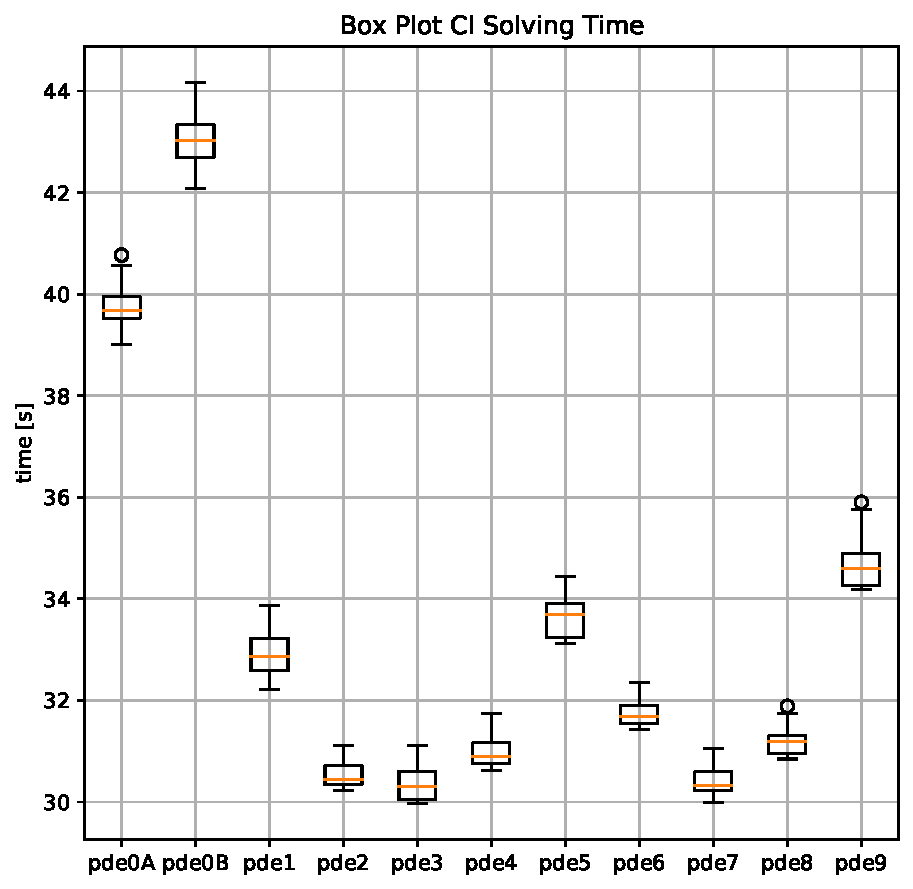
\includegraphics[width=\textwidth]{../../code/experiments/experiment_2/time_boxplot_ci_exp2.pdf}
	}
	\unterschrift{Solving time of the paJADE algorithm at $10^4$ \gls{nfe}}{}{}
	\label{fig:pajade_time_boxplot}
\end{figure}


\begin{figure}[H]
	\centering
	\noindent\adjustbox{max width=0.66\linewidth}{
		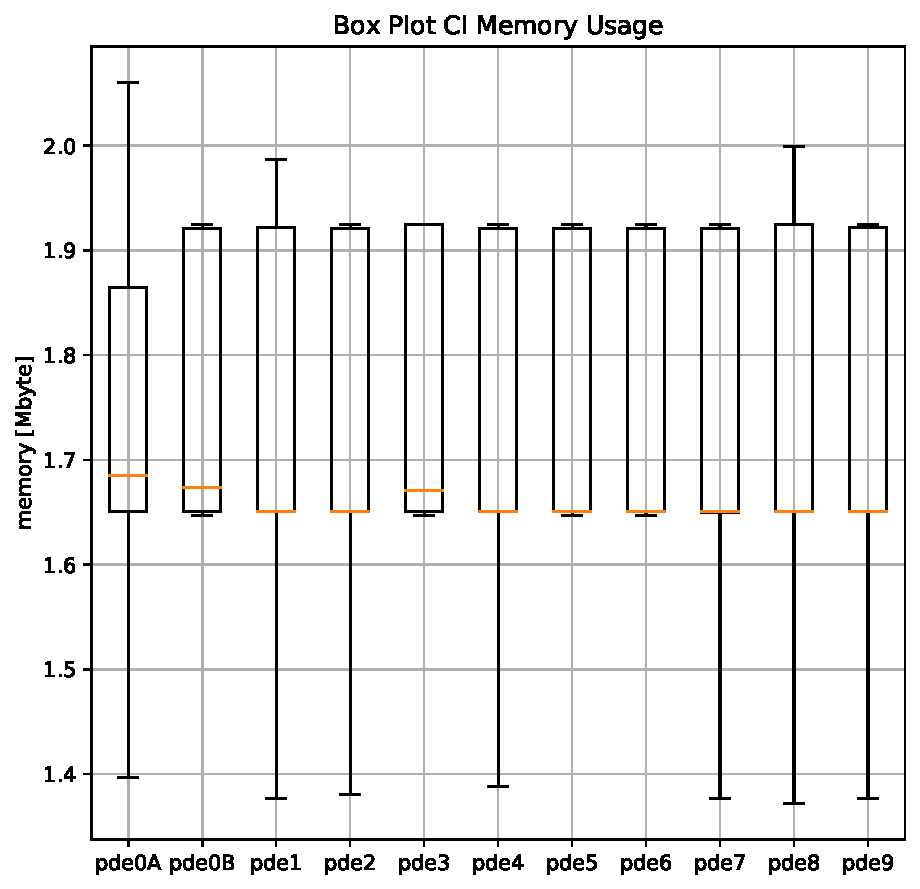
\includegraphics[width=\textwidth]{../../code/experiments/experiment_2/mem_boxplot_ci_exp2.pdf}
	}
	\unterschrift{Memory consumption of the paJADE at $10^4$ \gls{nfe}}{}{}
	\label{fig:pajade_memory_boxplot}
\end{figure}

\begin{table}[H]
	\centering
	\noindent\adjustbox{max width=\linewidth}{
		\begin{tabular}{|c|c|c|c|c|l|}
			
			\hline
			\rowcolor[HTML]{\farbeTabA}
			
			algorithm & \multicolumn{2}{|c|}{parallel JADE} & \multicolumn{2}{|c|}{adaptive JADE} & \\ \hline
			stat & mean & median & mean & median & Wilcoxon Test \\ \hline \hline
			\gls{pde} 0A & 0.6939 $\pm$ 0.6635 & 0.9243 & 9.6944E-16 $\pm$ 1.4867E-16 & 9.2559E-16 & sig. better \\ \hline
			\gls{pde} 0B & 0.2809 $\pm$ 0.3071 & 0.2035 & 0.2380 $\pm$ 0.0572 & 0.2607 & unsig. undecided \\ \hline
			\gls{pde} 1 & 0.0239 $\pm$ 0.0467 & 0.0146 & 0.0116 $\pm$ 0.0061 & 0.0084 & unsig. better \\ \hline
			\gls{pde} 2 & 0.0300 $\pm$ 0.0157 & 0.0255 & 0.0735 $\pm$ 0.0358 & 0.1034 & sig. worse \\ \hline
			\gls{pde} 3 & 0.0371 $\pm$ 0.0206 & 0.0295 & 0.1731 $\pm$ 0.0395 & 0.1822 & sig. worse \\ \hline
			\gls{pde} 4 & 0.0505 $\pm$ 0.0121 & 0.0481 & 0.0707 $\pm$ 0.0053 & 0.0720 & sig. worse\\ \hline
			\gls{pde} 5 & 1.2030 $\pm$ 0.0465 & 1.2053 & 122.6312 $\pm$ 372.5676 & 1.1643 & unsig. undecided \\ \hline
			\gls{pde} 6 & 0.5814 $\pm$ 1.3550 & 0.0000 & 0.4428 $\pm$ 1.0980 & 0.0000 & unsig. undecided \\ \hline
			\gls{pde} 7 & 0.0228 $\pm$ 0.0025 & 0.0226 & 0.0513 $\pm$ 0.0442 & 0.0231 & sig. worse \\ \hline
			\gls{pde} 8 & 0.2167 $\pm$ 0.0017 & 0.2169 & 0.2144 $\pm$ 0.0044 & 0.2128 & unsig. better \\ \hline
			\gls{pde} 9 & 0.0426 $\pm$ 0.0115 & 0.0463 & 0.0483 $\pm$ 0.0149 & 0.0468 & unsig. worse \\ \hline
			
		\end{tabular}
	}
	\unterschrift{Comparison of the achieved L2 norm by the pJADE and the paJADE at $10^6$ \gls{nfe}.}{}{}
	\label{tab:compare_mpj_mpja_10^6}
\end{table}




\section{Discussion}



\end{document}